\documentclass[oneside, abstracton, titlepage]{scrartcl}

\usepackage[left=2.5cm,right=2.6cm,top=3cm,bottom=3cm]{geometry}
\usepackage[utf8]{inputenc}
\usepackage[intlimits]{amsmath}
\usepackage{amssymb}
\usepackage{color}
\usepackage{xcolor}
\usepackage{subcaption}
\usepackage[version=4]{mhchem}

\usepackage{graphicx}

\newsavebox{\selvestebox}
\newenvironment{colbox}[1]
{\newcommand\colboxcolor{#1}%
	\begin{lrbox}{\selvestebox}%
		\begin{minipage}{\dimexpr\columnwidth-2\fboxsep\relax}}
		{\end{minipage}\end{lrbox}%
	\begin{center}
		\colorbox[HTML]{\colboxcolor}{\usebox{\selvestebox}}
\end{center}}
\newcommand\restr[2]{{% we make the whole thing an ordinary symbol
		\left.\kern-\nulldelimiterspace % automatically resize the bar with \right
		#1 % the function
		\vphantom{\big|} % pretend it's a little taller at normal size
		\right|_{#2} % this is the delimiter
}}

\begin{document}
	\title{Discovering governing reactions from concentration data}
	\maketitle

	\section{Introduction}
	When presented with a time series of possibly noisy non-equilibrium concentration fluctuations of some species as output of, e.g., measurements from experiments or simulations that were parameterized by microscopic rates, one can ask for the corresponding macroscopic rates and a generating reaction network.
	In this paper we present an application of the shallow learning method SINDy \cite{Brunton2015}. By sparse regression, it is able to identify generating nonlinear dynamics in data that stems from dynamical systems. The parsimonious nature of the results avoids overfitting and provides interpretability.
	In our application we, as opposed to the original method, do not only look for macroscopic rates of net species change but investigate the specific reactions that might have lead to the observations.
	We demonstrate the algorithm on two toy problems - one problem showing that when there is no ambiguity in the system, one converges to the correct rates with increasing resolution of concentration fluctuations and one in which we compute a sparse reaction network for given data.

	\section{The method}
	The underlying model is a law of mass action type dynamical system. To this end, let $S$ be the number of species, then the observed concentration at a time $t$ can be represented by a vector
	\begin{align}
	\mathbf{x}(t)=\begin{pmatrix}
	x_1(t)\\ \vdots \\ x_S(t)
	\end{pmatrix}\in \mathbb{R}^S.
	\end{align}
	Further, one can choose $R$ possible ansatz reactions with their respective reaction function
	\begin{align}
	\textbf{y}_r(\textbf{x}(t))=\begin{pmatrix}
	y_{r,1}(\textbf{x}(t)) \\ \vdots \\ y_{r,S}(\textbf{x}(t))
	\end{pmatrix}
	\end{align}
	so that the change of concentration for species $i$ at time $t$, is represented by the dynamical system
	\begin{align}
	\dot{\textbf{x}}_i(t) = \sum_{r=1}^{R}y_{r,i}(\textbf{x}(t))\xi_r,\quad i=1,\ldots, S,
	\label{method:the-system}\end{align}
	where $\xi_r$ are the to-be estimated macroscopic rates.

	When presented with a time series consisting of $T$ observations, the data can be represented as a matrix
	\begin{align}
	\textbf{X} = \begin{pmatrix}
		x_1(t_1) & x_2(t_1) & \cdots & x_S(t_1) \\
		x_1(t_2) & x_2(t_2) & \cdots & x_S(t_2) \\
		\vdots   & \vdots   & \ddots & \vdots   \\
		x_1(t_T) & x_2(t_T) & \cdots & x_S(t_T)
	\end{pmatrix} \in \mathbb{R}^{T\times S}.
	\end{align}
	Given this matrix, one can propose a library $\Theta(\textbf{X}) = \begin{pmatrix} \theta_1(\textbf{X}) & \theta_2(\textbf{X}) & \cdots & \theta_R(\textbf{X}) \end{pmatrix}$ of $R$ ansatz reactions with corresponding reaction functions
	\begin{align}
		\theta_r(\textbf{X}) = \begin{pmatrix}
		\textbf{y}_r(\textbf{X}_1)^T \\ \vdots \\ \textbf{y}_r(\textbf{X}_T)^T
		\end{pmatrix}\in \mathbb{R}^{T\times S},\quad r=1,\ldots,R,
	\label{method:the-reactions}\end{align}
	where $\textbf{X}_i$ denotes the $i$-th row in $X$. Applying the concentration trajectory to the library yields $\Theta(\textbf{X})\in\mathbb{R}^{T\times S\times R}$. Following the approach of SINDy, the goal is to find coefficients $\Xi = \begin{pmatrix} \xi_1 & \xi_2 & \cdots & \xi_R
	\end{pmatrix}^T$, so that
	\begin{align}
	\dot{\textbf{X}} = \Theta(\textbf{X})\Xi = \sum_{r=1}^{R}\theta_r(\textbf{X})\xi_r.
	\end{align}
	In particular, the system is linear in the coefficients $\Xi$, which makes potentially sparse regression tools such as elastic net regularization \cite{Zou2005} applicable. To this end, one can consider the minimization problem to find $\hat{\Xi}$ such that
	\begin{align}
		\hat{\Xi} = \underset{\Xi}{\arg\min}\left( \frac{1}{2T}\left\| \dot{\textbf{X}} - \Theta(\textbf{X})\Xi \right\|_F^2 + \alpha\lambda\|\Xi\|_1 + \alpha(1-\lambda)\|\Xi\|_2^2 \right) \quad \text{subject to }\Xi \geq 0,
	\label{method:minimizationproblem}\end{align}
	where $\|\cdot\|_F$ denotes the Frobenius norm, $\lambda\in[0,1]$ a hyperparameter that interpolates linearly between LASSO \cite{Tibshirani1996, Hastie2009} and Ridge \cite{Hoerl1} methods, and $\alpha\geq 0$ is a hyperparameter that, depending on $\lambda$, can induce sparsity and give preference to smaller solutions in the $L_1$ or $L_2$ sense.

	When presented with multiple trajectories one can extend the objective function by a sum over these and obtain a more general minimization problem that reads: Find $\hat{\Xi}$ such that
	\begin{align}
		\hat{\Xi} = \underset{\Xi}{\arg\min}\left( \sum_{\text{traj}}\frac{1}{2T_{\text{traj}}}\left\| \dot{\textbf{X}}_\text{traj} - \Theta(\textbf{X}_\text{traj})\Xi \right\|_F^2 + \alpha\lambda\|\Xi\|_1 + \alpha(1-\lambda)\|\Xi\|_2^2 \right)
	\end{align}
	subject to $\Xi\geq 0$.
	For $\alpha=0$ the minimization problem reduces to constrained least-squares. In order to solve (\ref{method:minimizationproblem}) the sequential least-squares minimizer SLSQP \cite{Kraft1988} is applied via the software package SciPy \cite{SciPy}. Since only the concentration data $\mathbf{X}$ is available but not its temporal derivative $\dot{\mathbf{X}}$, it is approximated numerically by second order finite differences with the exception of boundary data.

    \section{Example system: Regulation of gene expression}\label{sec:generegulation}

    To demonstrate the method a gene-regulatory network is estimated from time series of molecule-concentrations. The data of is generated by integrating the law of mass action equations of the underlying model and adding Gaussian noise.
    
    To this end, let $A$, $B$, and $C$ be three species of proteins which are being translated from a corresponding mRNA molecule. Each mRNA in turn has a corresponding DNA which it is transcribed from. The proteins and mRNA molecules decay over time whereas the DNA concentration remains constant.
    
    For each of the three species one can formulate the following basic reactions
	\begin{align*}
        \ce{ DNA_i } & \ce{ -> DNA_i + mRNA_i } &\text{(transcription)}, \\
        \ce{ mRNA_i } & \ce{ -> mRNA_i + Protein_i } &\text{(translation)}, \\
        \ce{ mRNA_i } & \ce{ -> } \emptyset &\text{(decay of mRNA)}, \\
        \ce{ Protein_i } & \ce{ -> } \emptyset &\text{(decay of Protein)},
    \end{align*}
    for $i=A,B,C$.

    The protein concentrations of $A$, $B$, and $C$ regulate each other in a negative way by hindering the transcription process. In the law of mass action model we account for this by a reaction. A repression of species $j$ by species $i$ can be modeled as
    \begin{equation*}
        \ce{ Protein_i + mRNA_j -> Protein_i } \quad \text{(regulation by repression)}.
    \end{equation*}

    In our example proteins of type $A$ regulate the mRNA$_\mathrm{B}$ molecules, proteins of type $B$ regulate the mRNA$_\mathrm{A}$ molecules and proteins of type $C$ regulate the mRNA$_\mathrm{A}$ molecules. The network of all species and reactions is depicted in Figure \ref{fig:network}. This serves as reference model to generate the time series of concentrations.
    \begin{figure}
        \centering
        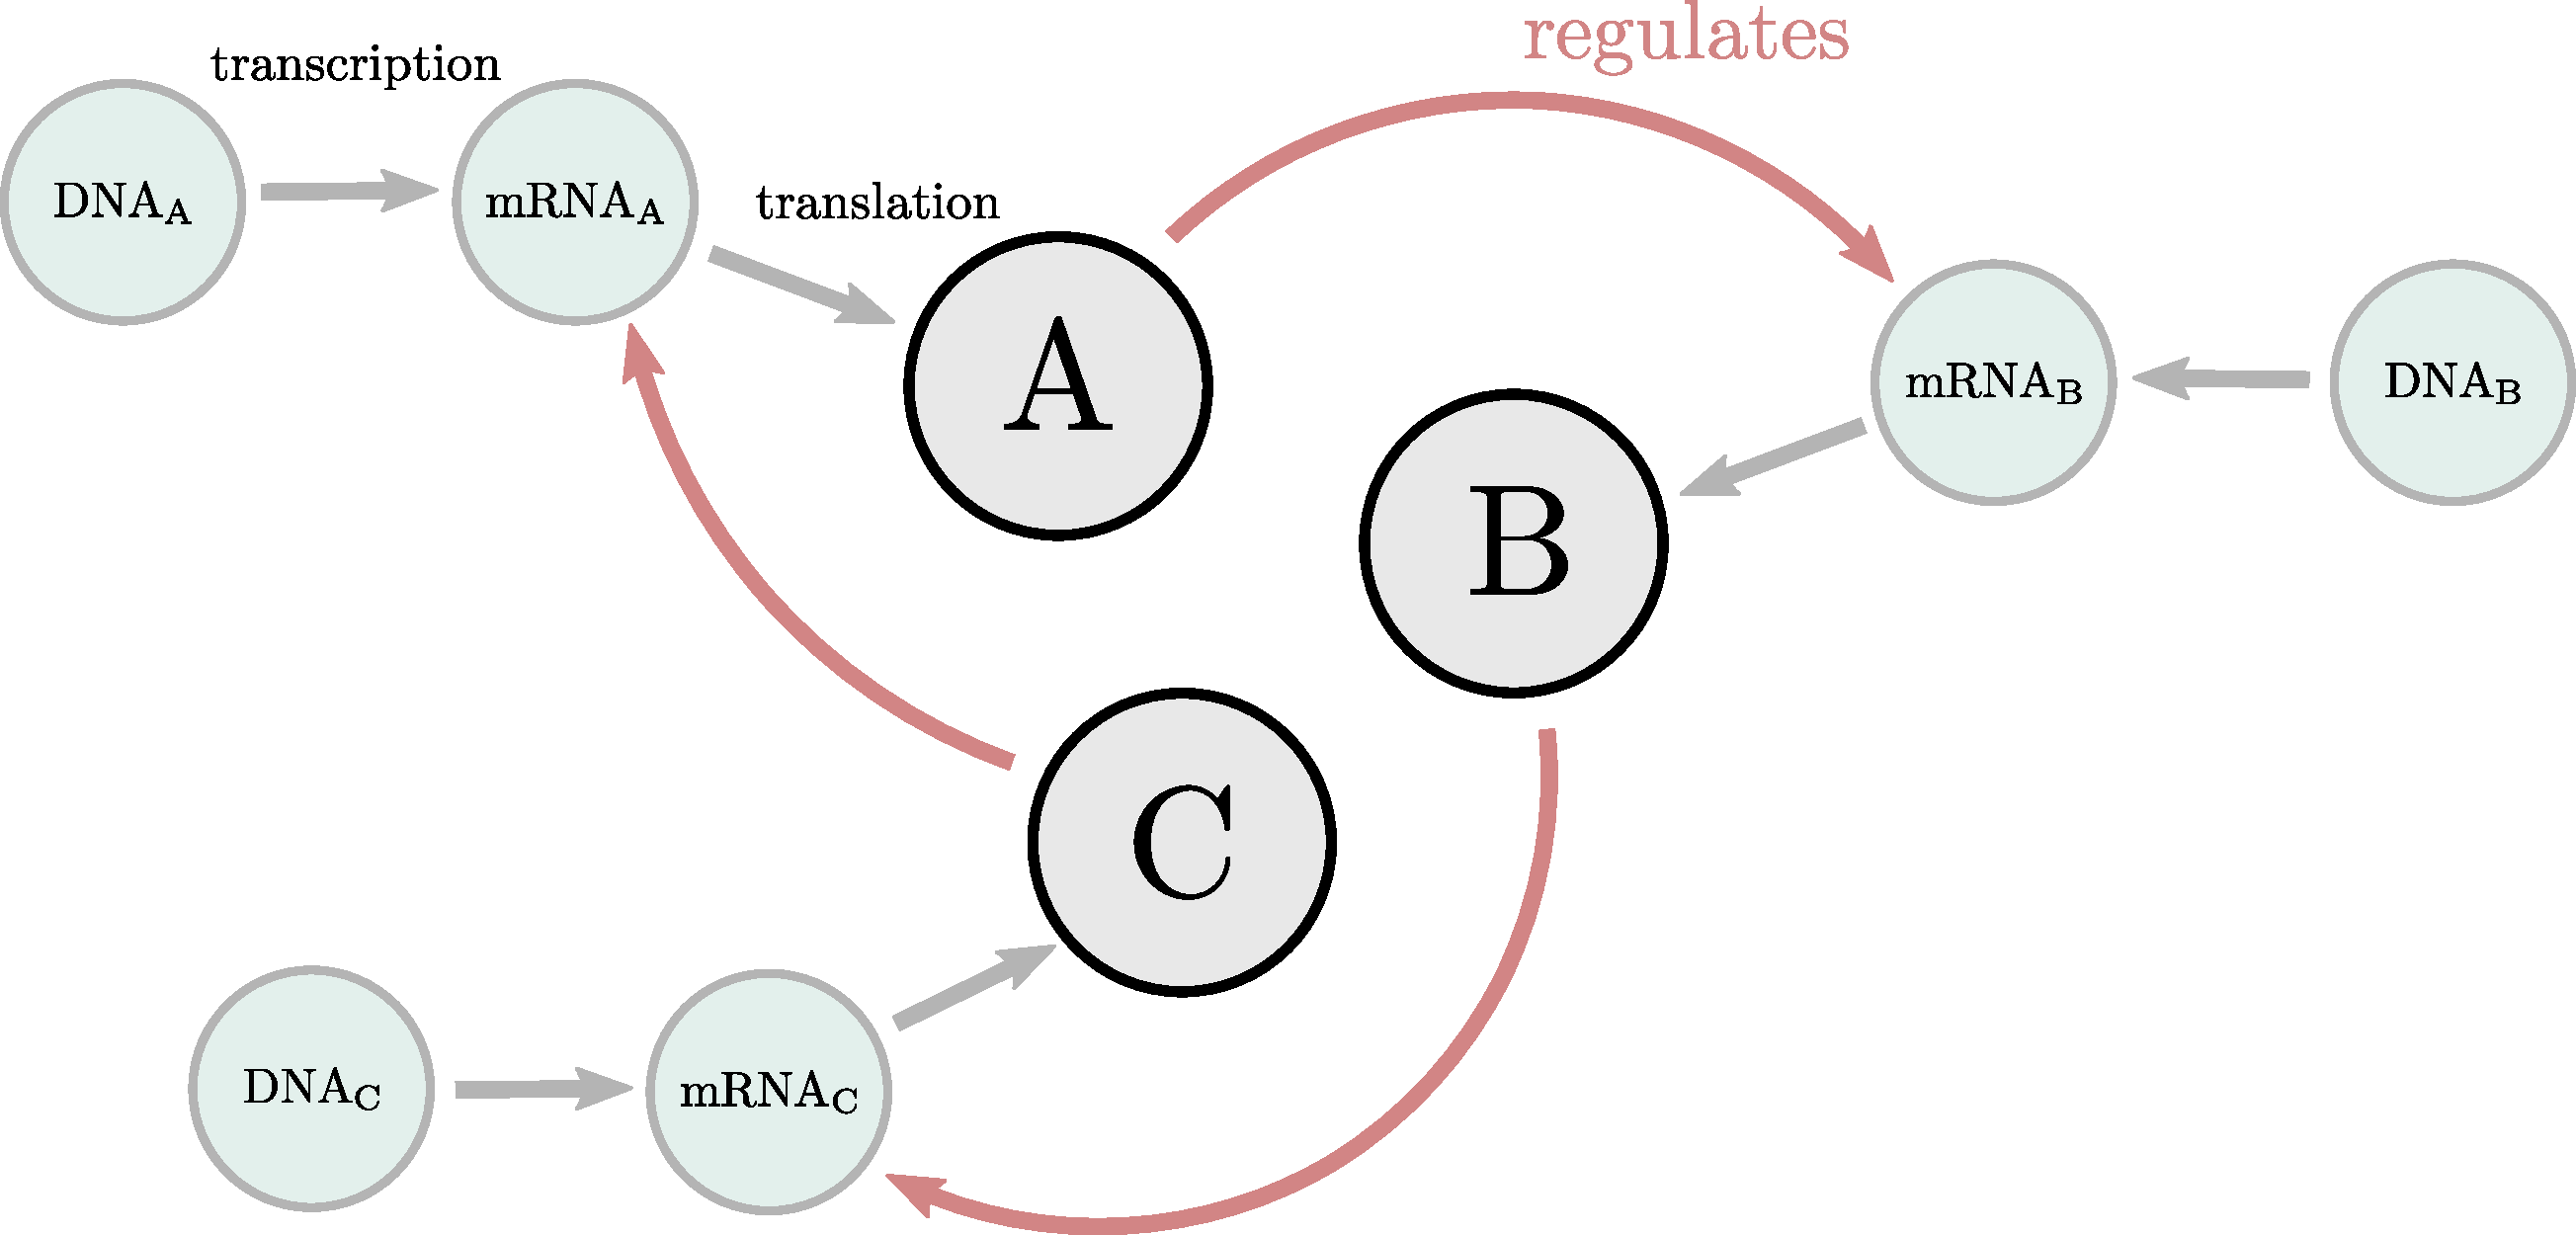
\includegraphics[width=.5\textwidth]{./figures_tex/gene_regulation_full.pdf}
        \caption{The regulation network example described in Section \ref{sec:generegulation}. Each circle depicts a species, each arrow corresponds to one reaction. The red arrows describe the regulatory network which generates the example data.}
        \label{fig:network}
    \end{figure}


    \section{Scenarios of measurement}\label{sec:scenarios-of-measurement}

    The proposed estimation method is designed to find reaction networks and rates from experimental data. In the following measurement scenarios are considered that differ in how many time series are available and the level of noise that the data is subject to:
    \begin{enumerate}
        \item The initial state of the measurement apparatus can be reproduced exactly. There is only one set of generating reaction rates. Each frame of a time series is subject to noise. The outcome of this scenario is one time series of concentrations with a certain noise-level.
        \item The process is observed multiple times. The initial state of the measurement apparatus differs in each observation. The outcome of this scenario is multiple time series each with a certain noise level and different initial states.
        \item The process is observed multiple times. The initial state of the measurement apparatus differs in each observation. Additionally the generating reaction rates differ slightly in each observation. The outcome of this scenario is multiple time series each with a given noise level, different initial states and slightly perturbed underlying reaction rates.
    \end{enumerate}


	\section{Examples}

	In the following two examples are presented. The first example considers data according to the first scenario of measurement as presented in Section \ref{sec:scenarios-of-measurement}.
	The minimization problem (\ref{method:minimizationproblem}) with $\alpha=0$ is solved for different magnitudes of noise variance.

	\subsection{Regression without regularization}
	\label{sec:ex1}

	In this example it is demonstrated that given enough data, the original model can be recovered in the limit of the noise variance $\sigma^2\to 0$.
	
	\begin{colbox}{F8E0E0}
		todo
	\end{colbox}
	
	Here we demonstrate that, with decreasing time step $\Delta t$ and $\alpha=0$, the estimated rates converge to the true rates if there is no ambiguity in the system. Let there be two species $A$ and $B$ which can unimolecularly convert into each other with macroscopic rates of $k_1=4.0$ and $k_2=0.5$, respectively. The initial amount of particles is set to $70$ of type $A$ and $0$ of type $B$. The law of mass action solution and Gillespie realization corresponding to this system are depicted in Figure \ref{ex1:concentration-curves}.

	\begin{figure}
		\begin{center}
			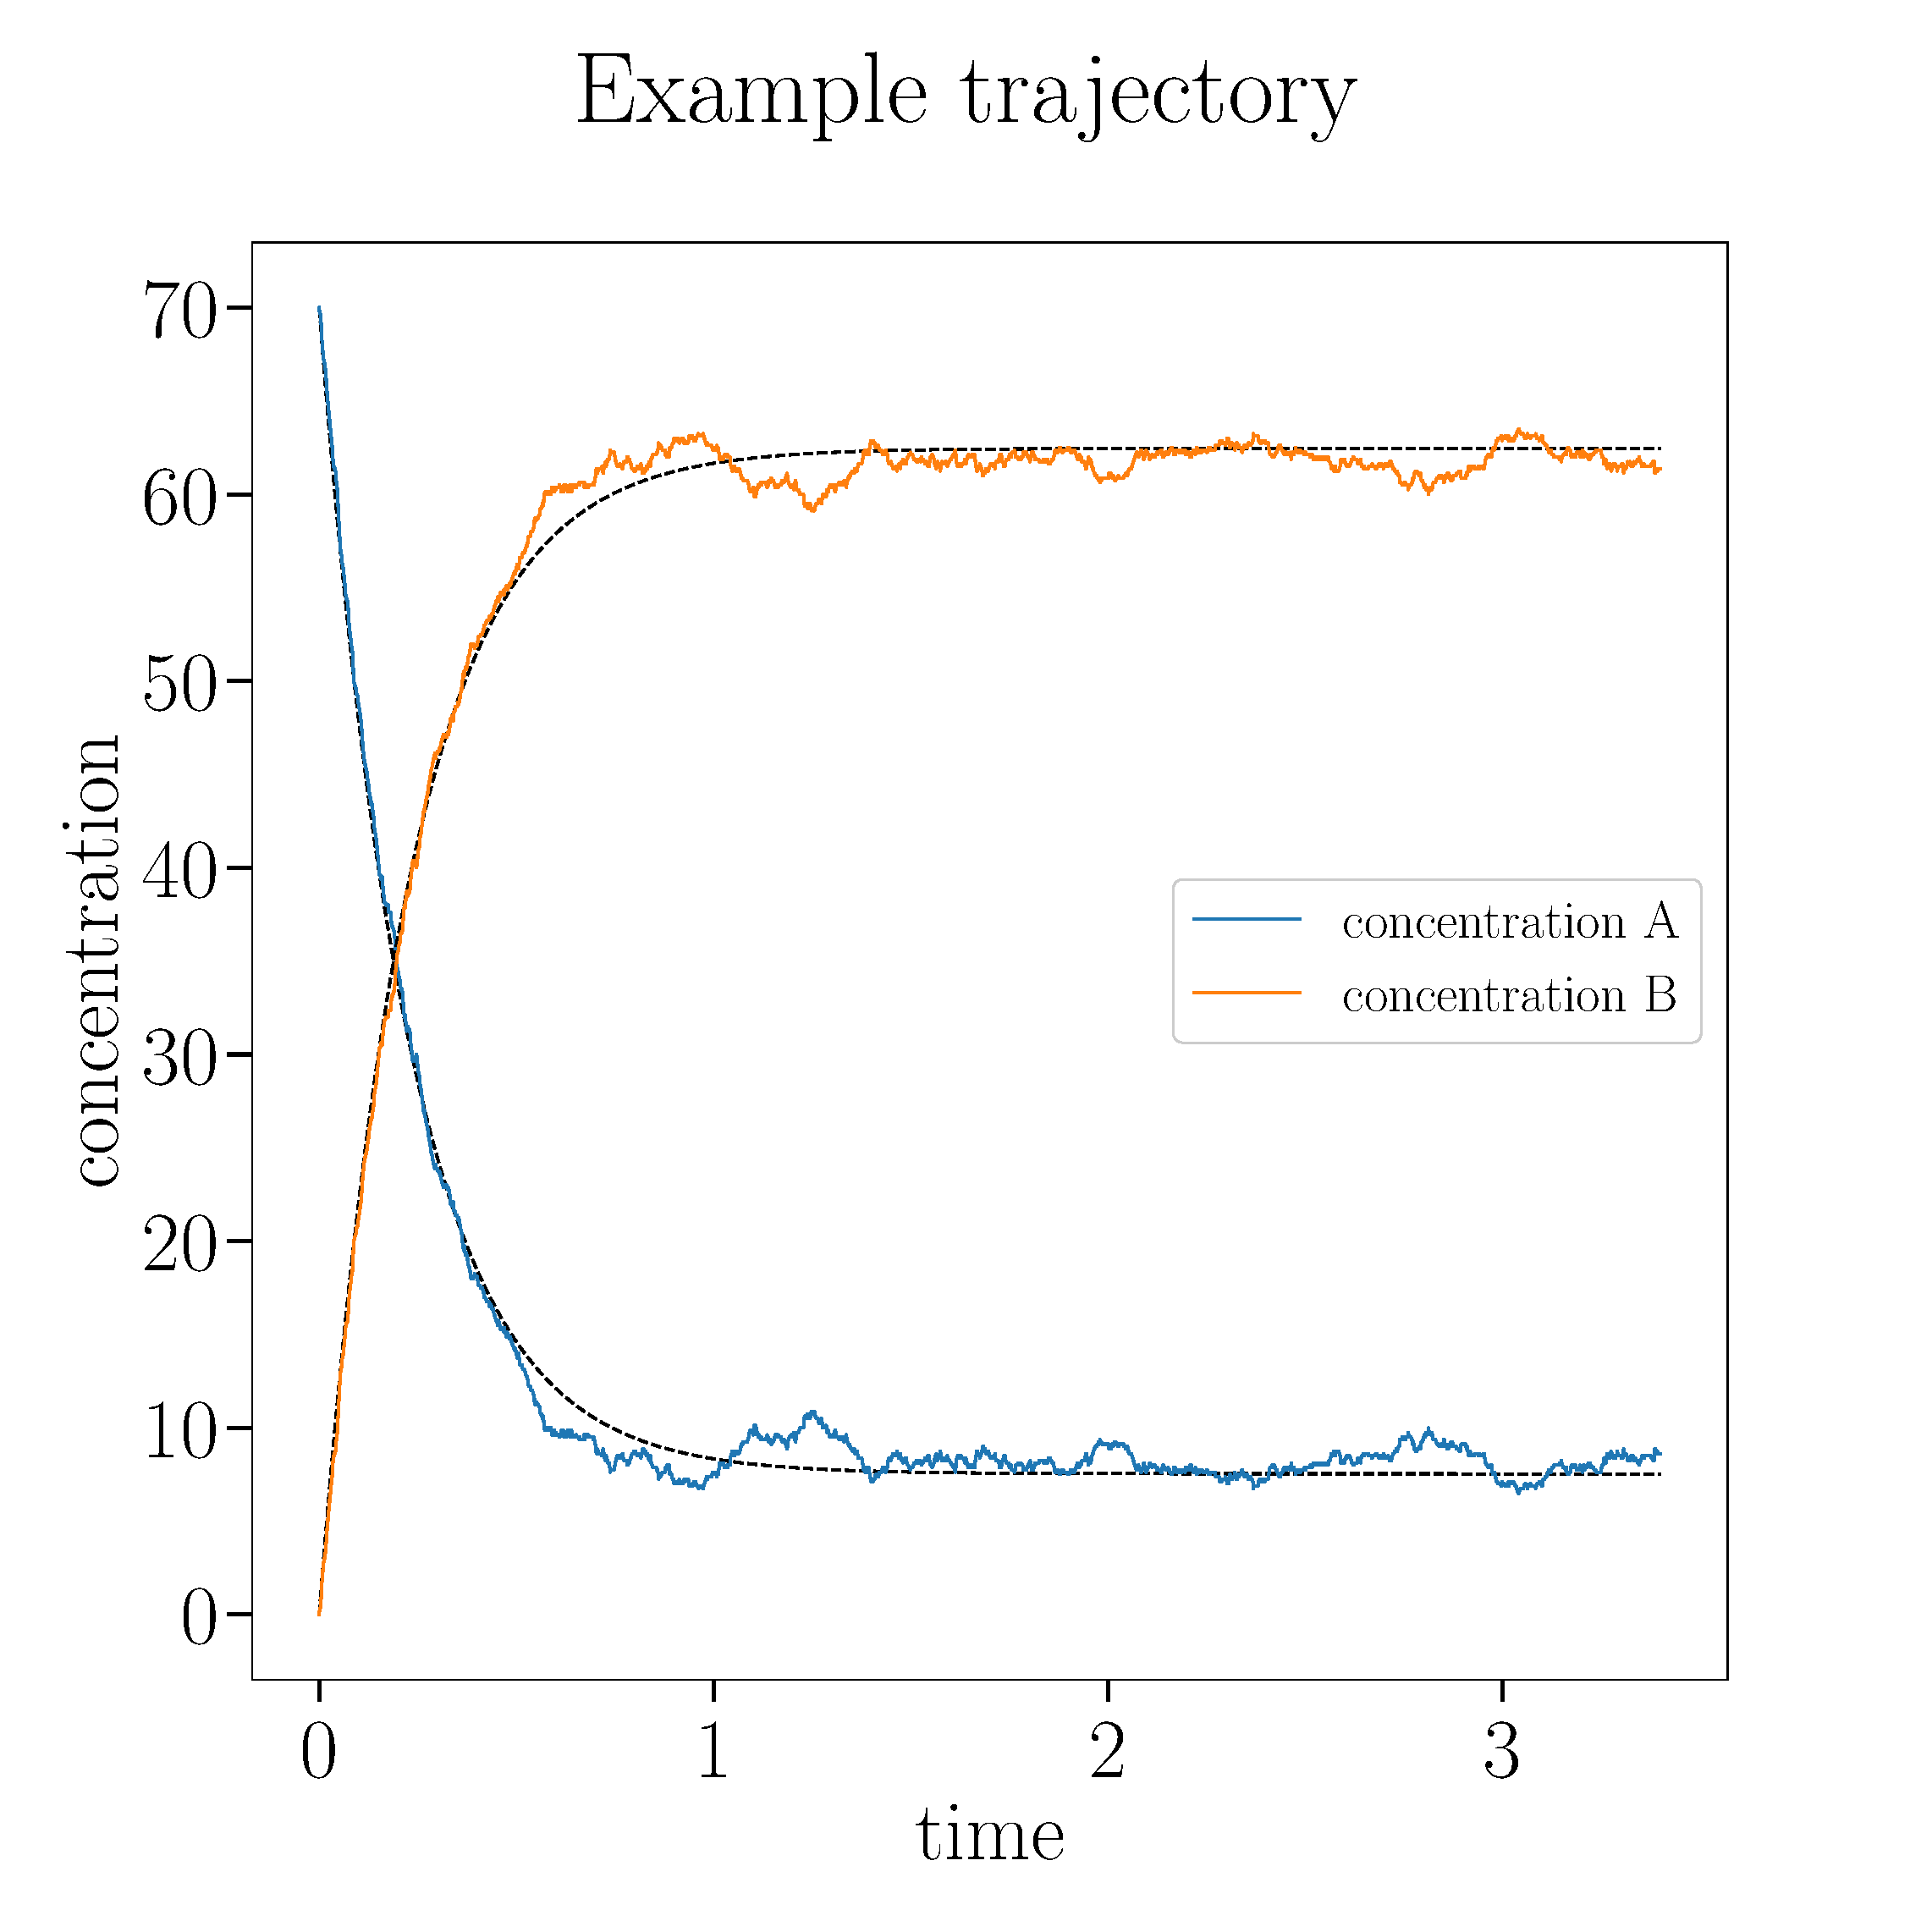
\includegraphics[width=.5\textwidth]{./figures_tex/aux_ex1_concentration_curves}
		\end{center}
		\caption{The law of mass action solution and a Gillespie realization of the example given in Section \ref{sec:ex1}.}
		\label{ex1:concentration-curves}
	\end{figure}

	For each $\Delta t$, eight different realizations with identical starting conditions are averaged into a single trajectory, of which then the rates for reactions $A\to B$ and $B\to A$ are estimated. This procedure was repeated $30$ times. In Figure \ref{ex1:rates-convergence}, the average estimates with their standard deviations are shown. One can see that, with decreasing $\Delta t$, the estimates become better and the rates can be recovered. Further it can be observed that in this case a time step of $\Delta t\approx 10^{-2}$ suffices.

	\begin{figure}
		\begin{center}
			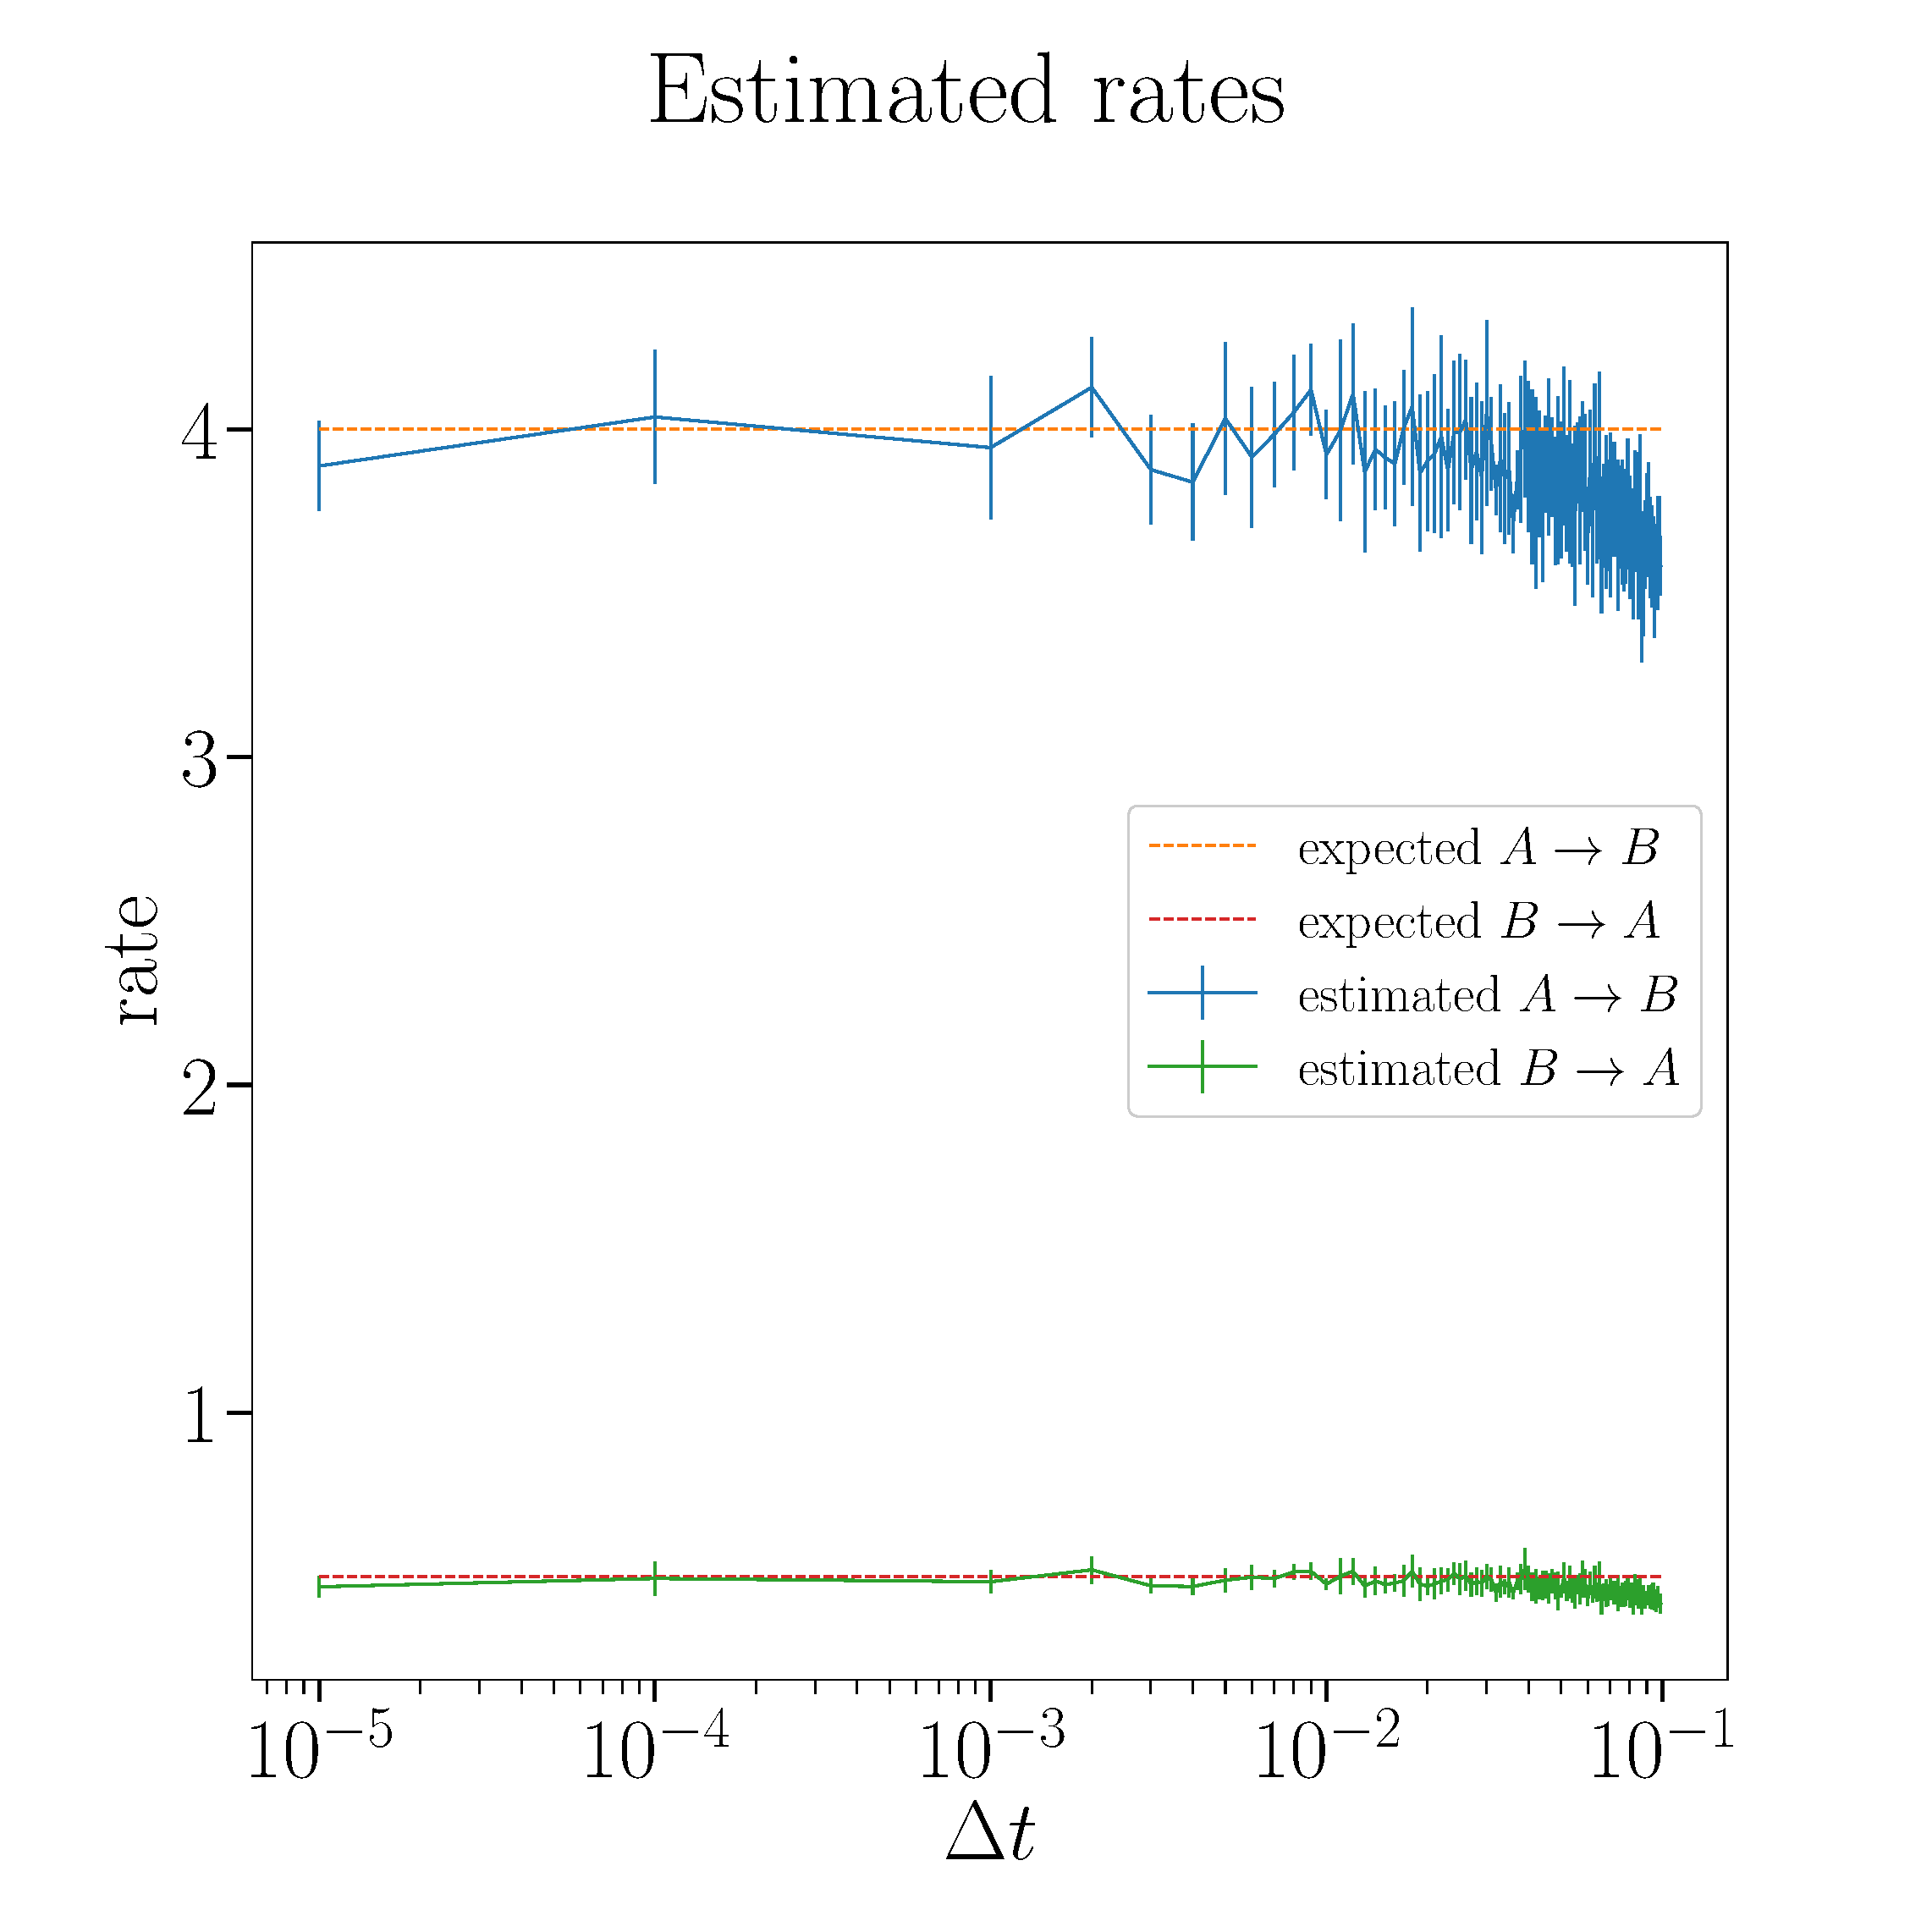
\includegraphics[width=.5\textwidth]{./figures_tex/aux_rates_convergence}
		\end{center}
		\caption{Convergence of estimated rates with decreasing $\Delta t$.}
		\label{ex1:rates-convergence}
	\end{figure}

	\subsection{Regression with regularization}
	\label{sec:ex2}
	In this example there are four species $A$, $B$, $C$, and $D$. The system was generated with reactions $A\xrightarrow{k_1}D$, $D\xrightarrow{k_2}A$, $D\xrightarrow{k_3}B$, $A+B\xrightarrow{k_4}C$, and $C\xrightarrow{k_5}D+B$, where the rates are given in Table \ref{tab:estimated-rates}. These reactions are inserted into the ansatz library $\Theta (\cdot)$. Additionally the reactions $A\leftrightarrow B$, $A\leftrightarrow C$, and $A+C\leftrightarrow D$ are inserted into the library.

	\begin{figure}
		\centering
		\begin{subfigure}[b]{.45\textwidth}
			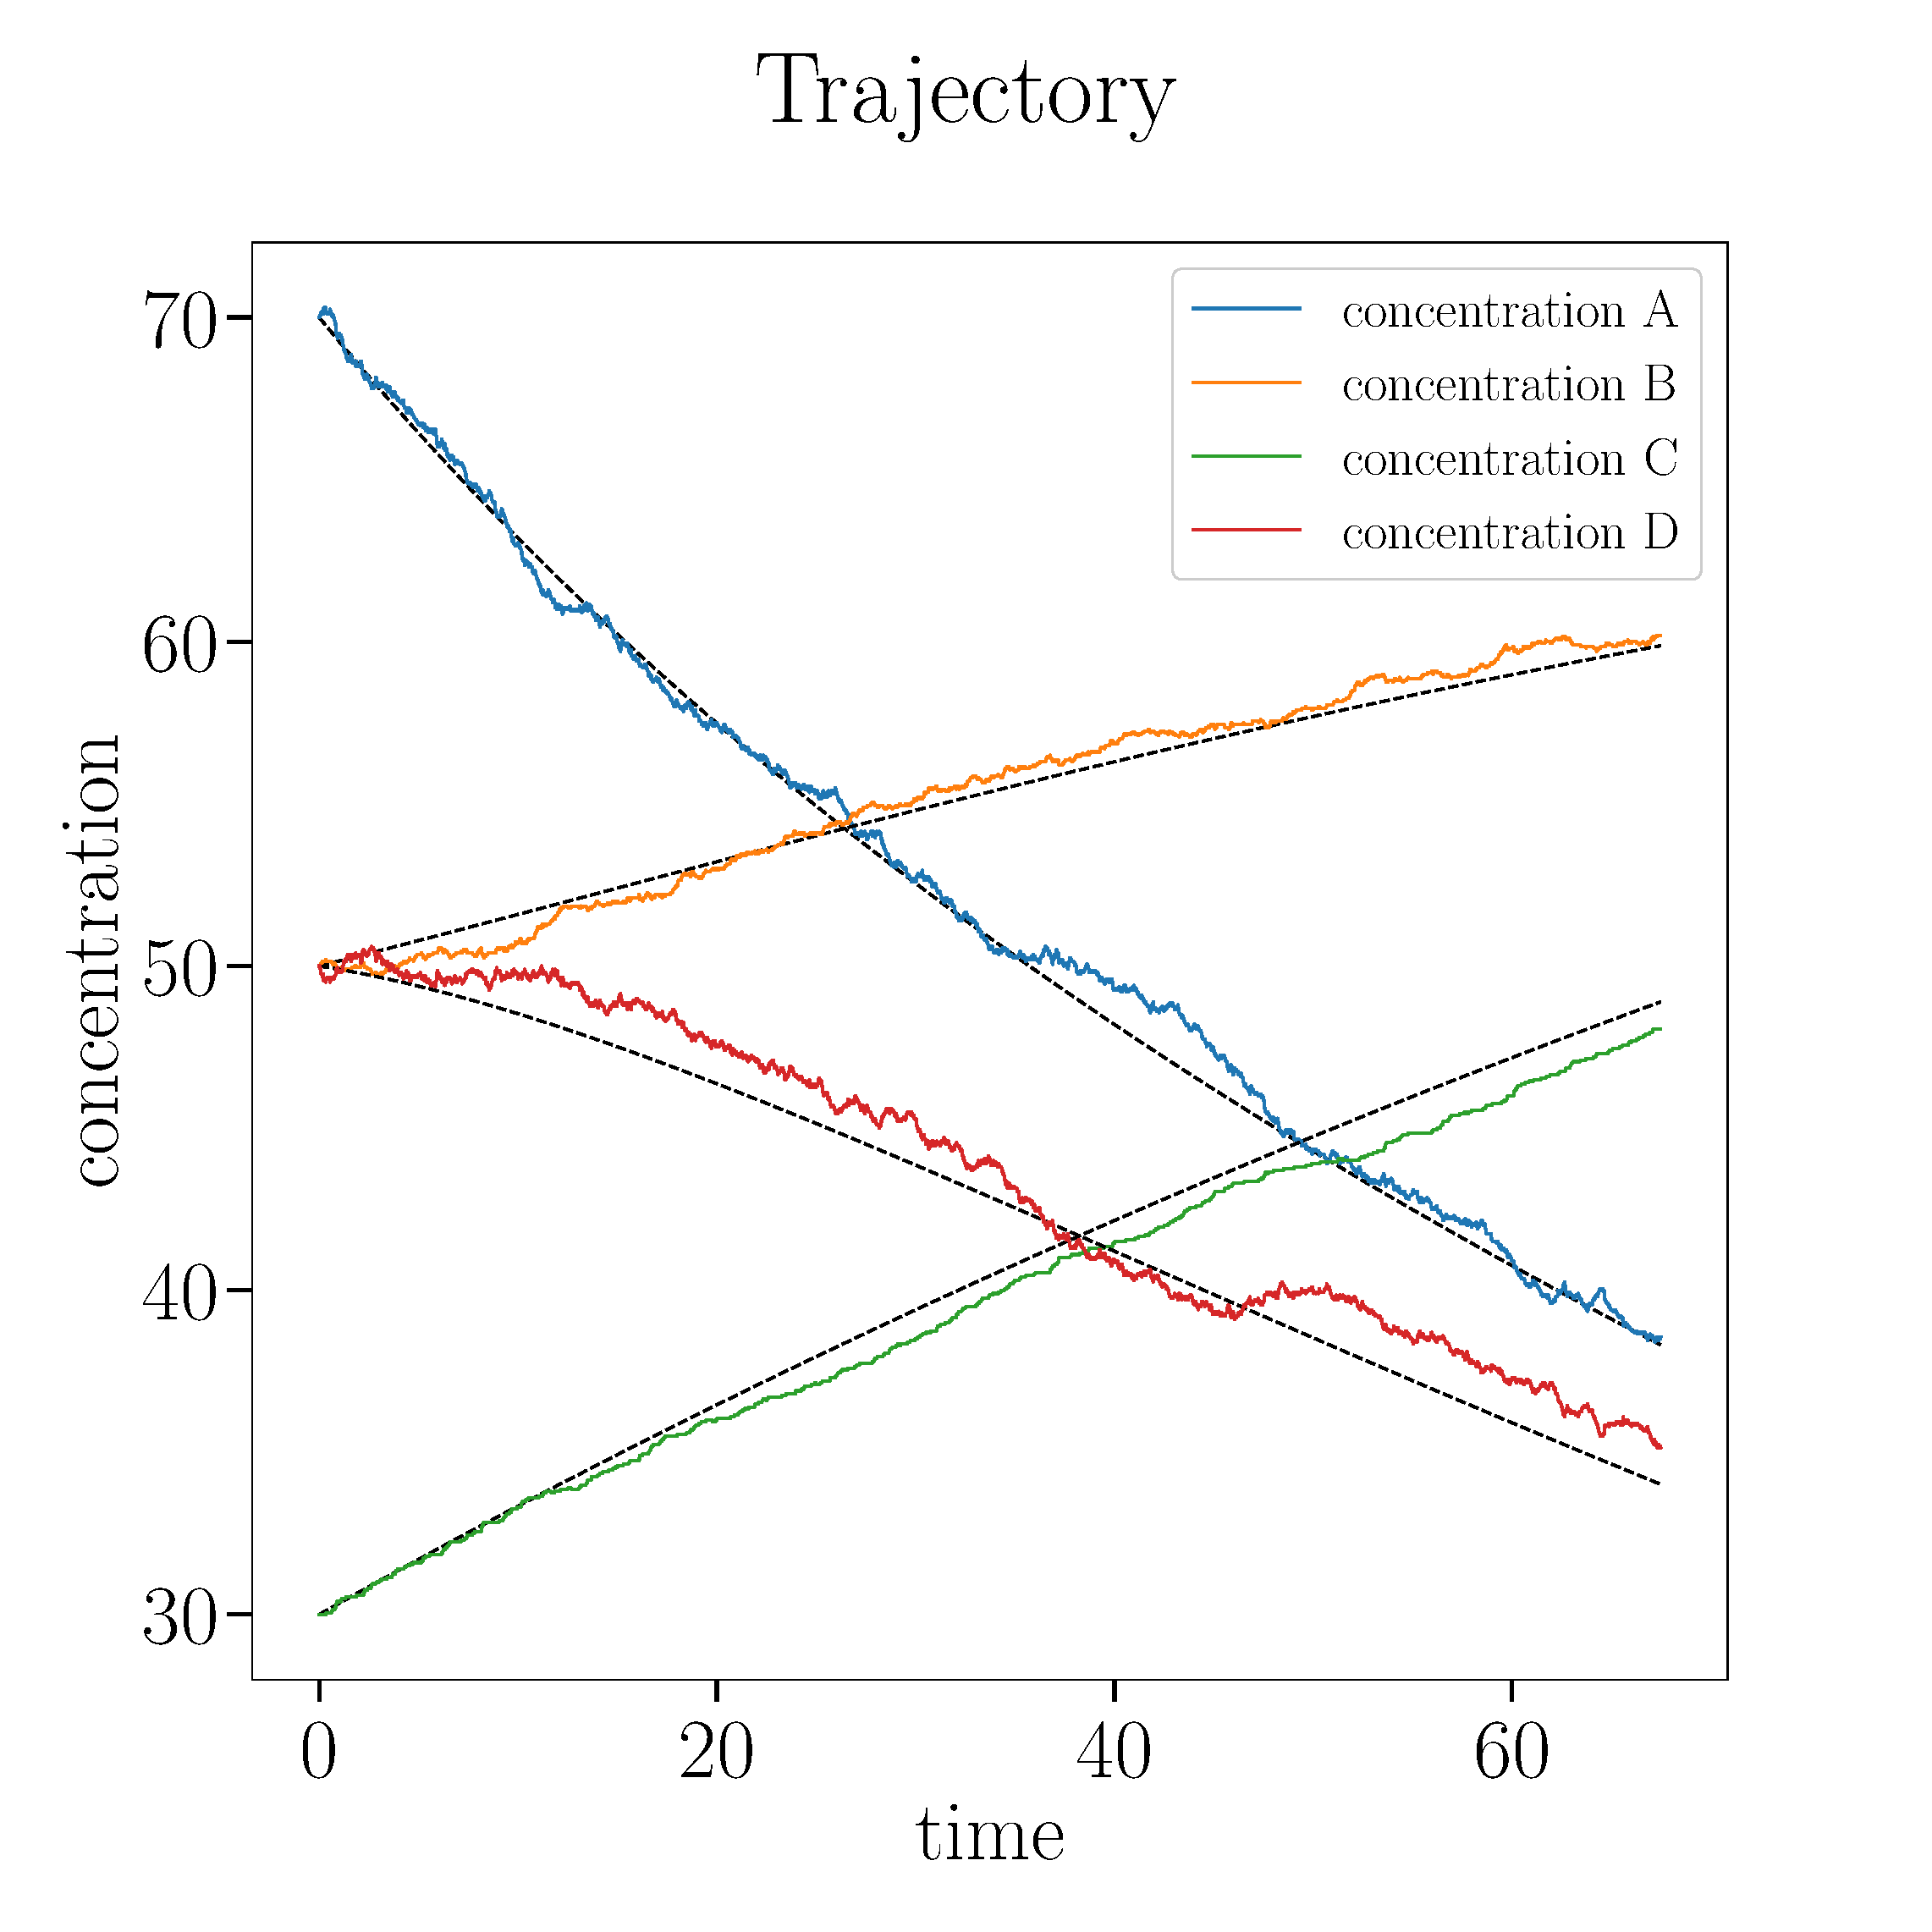
\includegraphics[width=\textwidth]{./figures_tex/cv_concentrations_train}
			\caption{Train data set.}
		\end{subfigure}
		~
		\begin{subfigure}[b]{.45\textwidth}
			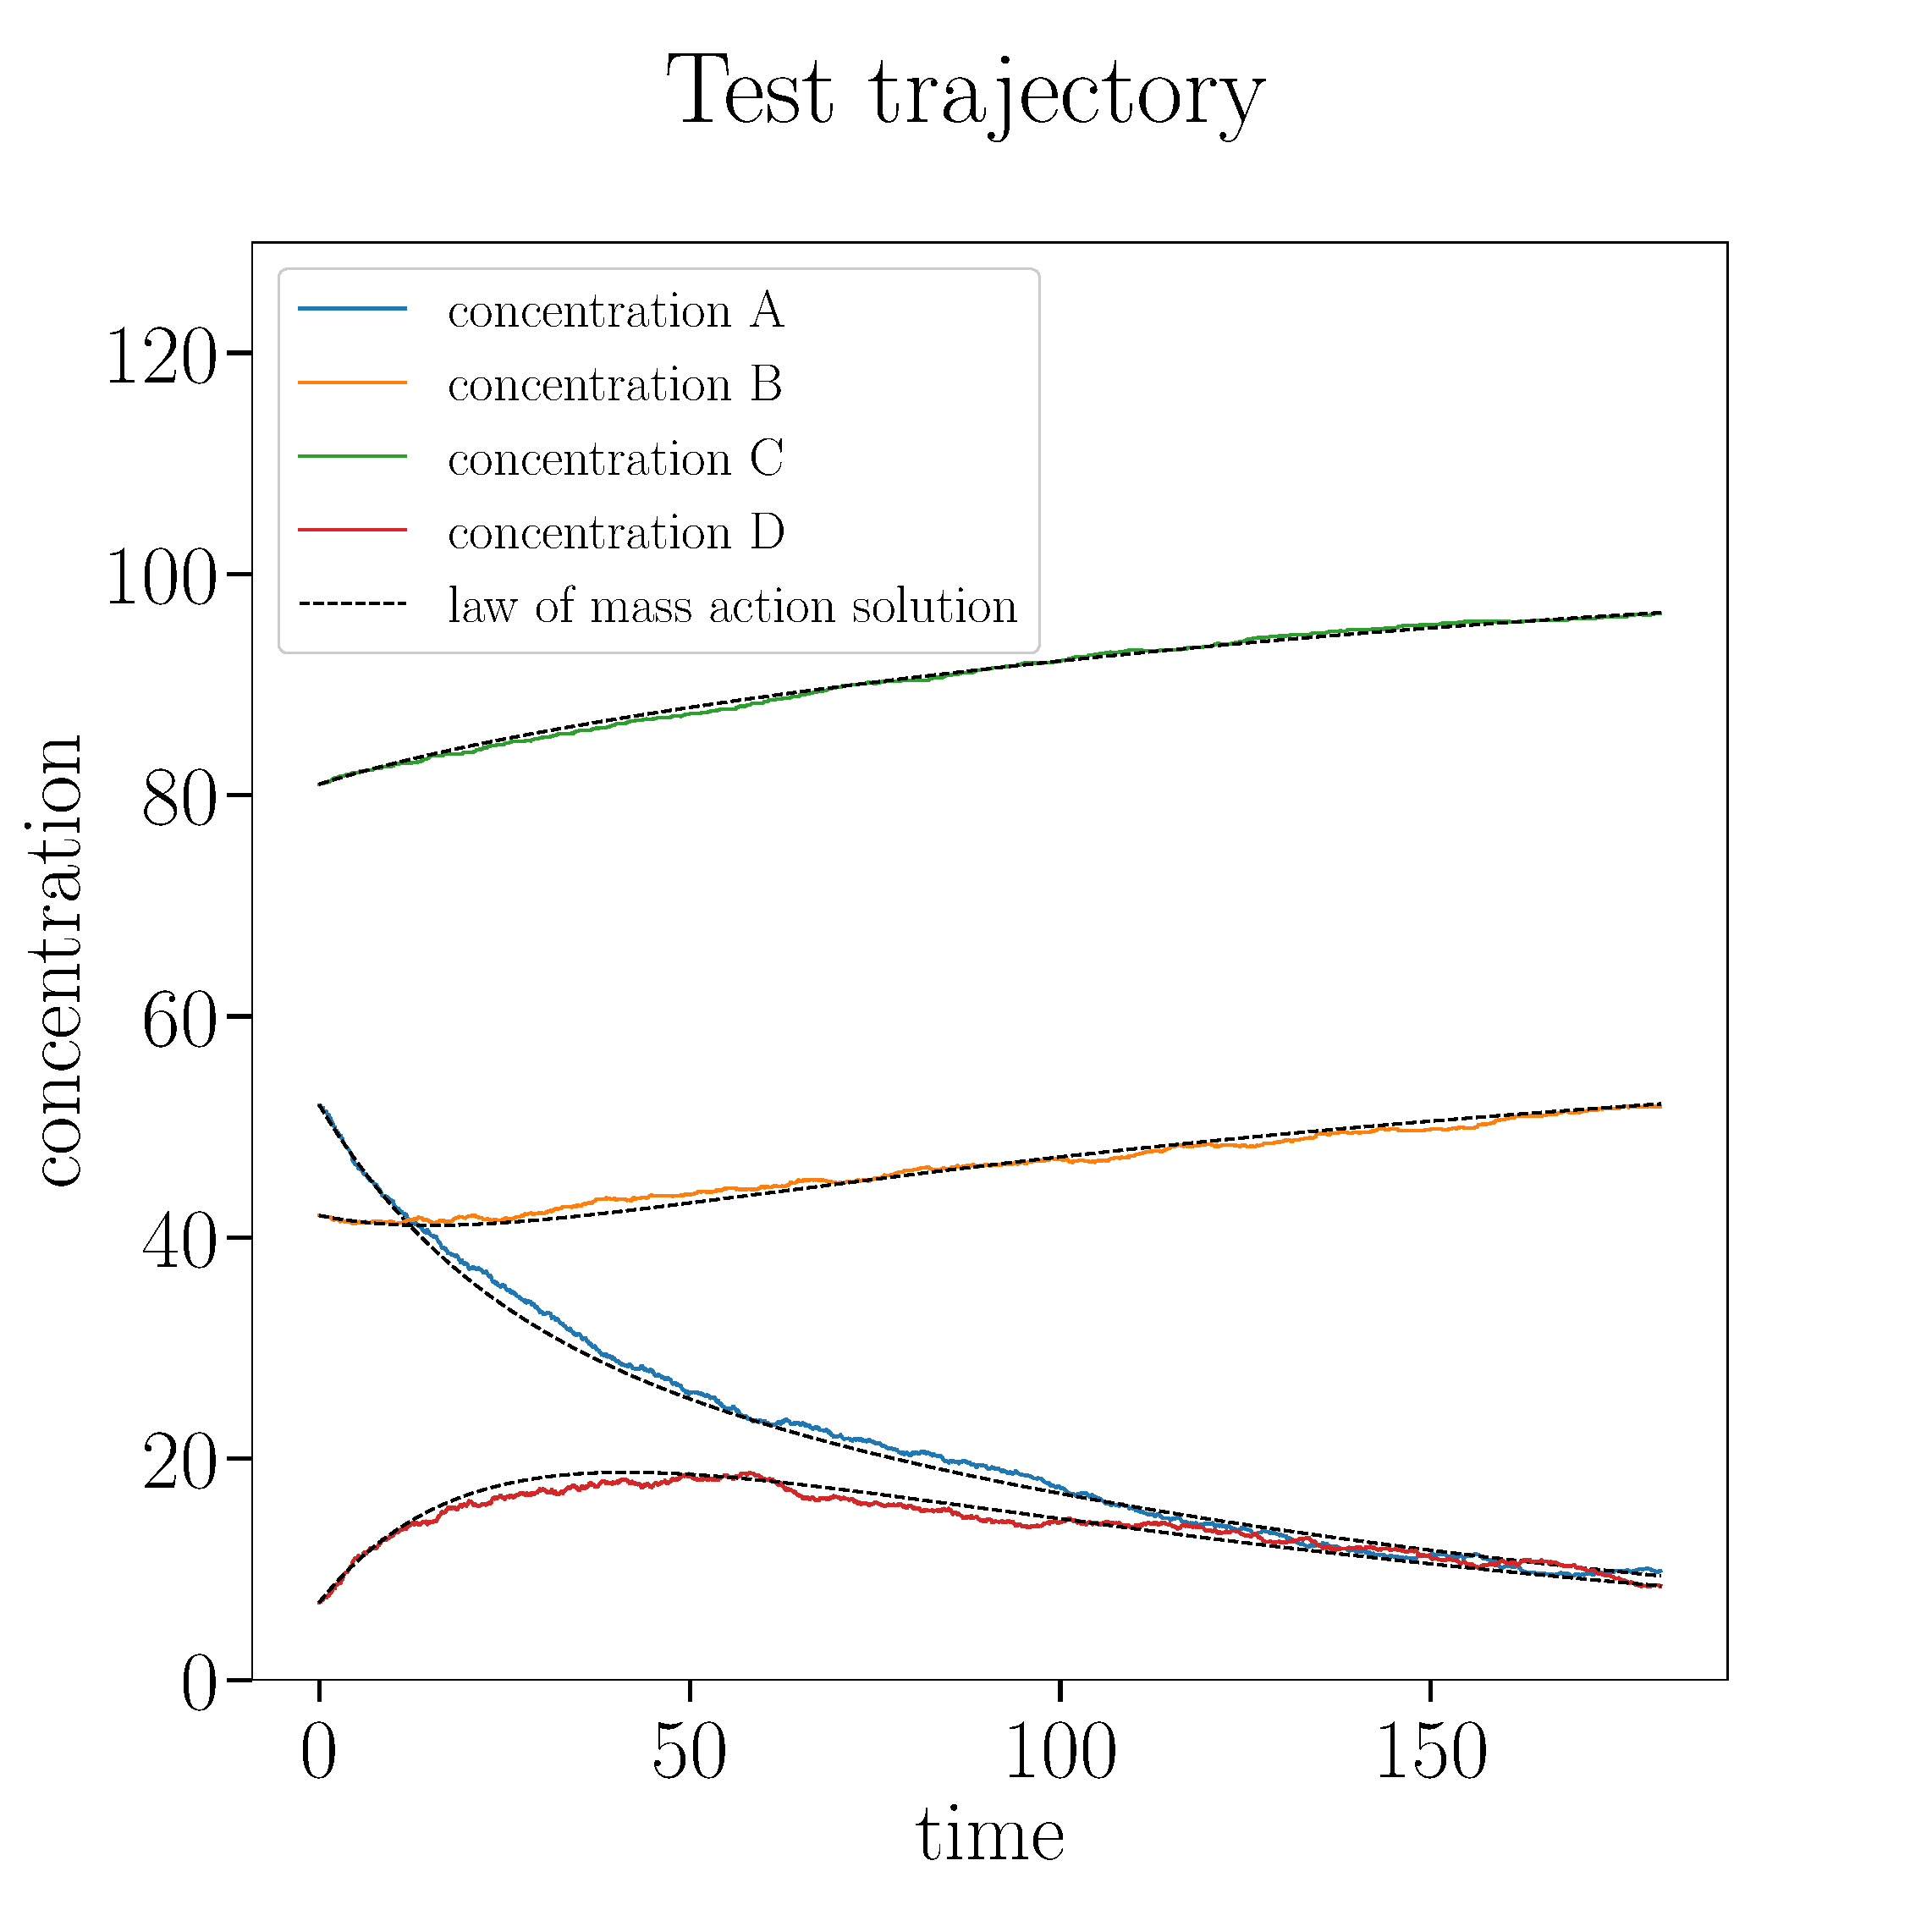
\includegraphics[width=\textwidth]{./figures_tex/cv_concentrations_test}
			\caption{Test data set.}
		\end{subfigure}
		\caption{Train and test data sets for the example given in Section \ref{sec:ex2}.}
		\label{ex2:test-train-concentration-curves}
	\end{figure}

	The problem now is to find a suitable $\alpha$ such that a parsimonious solution is yielded. To this end, cross-validation is applied. The trajectories that are used as training and test data set are depicted in Figure \ref{ex2:test-train-concentration-curves}. \textcolor{red}{Perhaps use several test trajectories with different initial conditions to get something like a confidence interval?} As an indicator to the estimation error one can use the scoring function
	\begin{align}
		f_\alpha = \frac{1}{T}\|\dot{\mathbf{X}}_\text{test} - \Theta (\textbf{X}_\text{test}) \Xi_\text{train}\|_F^2,
		\label{ex2:score-function}
	\end{align}
	where the best possible score is $f_\alpha = 0$ and larger values indicate worse models.
	For a selection of hyperparameters $\alpha\in [0, 100]$, the model parameters $\Xi$ are estimated and the scoring function (\ref{ex2:score-function}) evaluated, yielding a dependency of the score on $\alpha$ as depicted in Figure \ref{ex2:score-graph}.

	\begin{figure}
		\begin{center}
			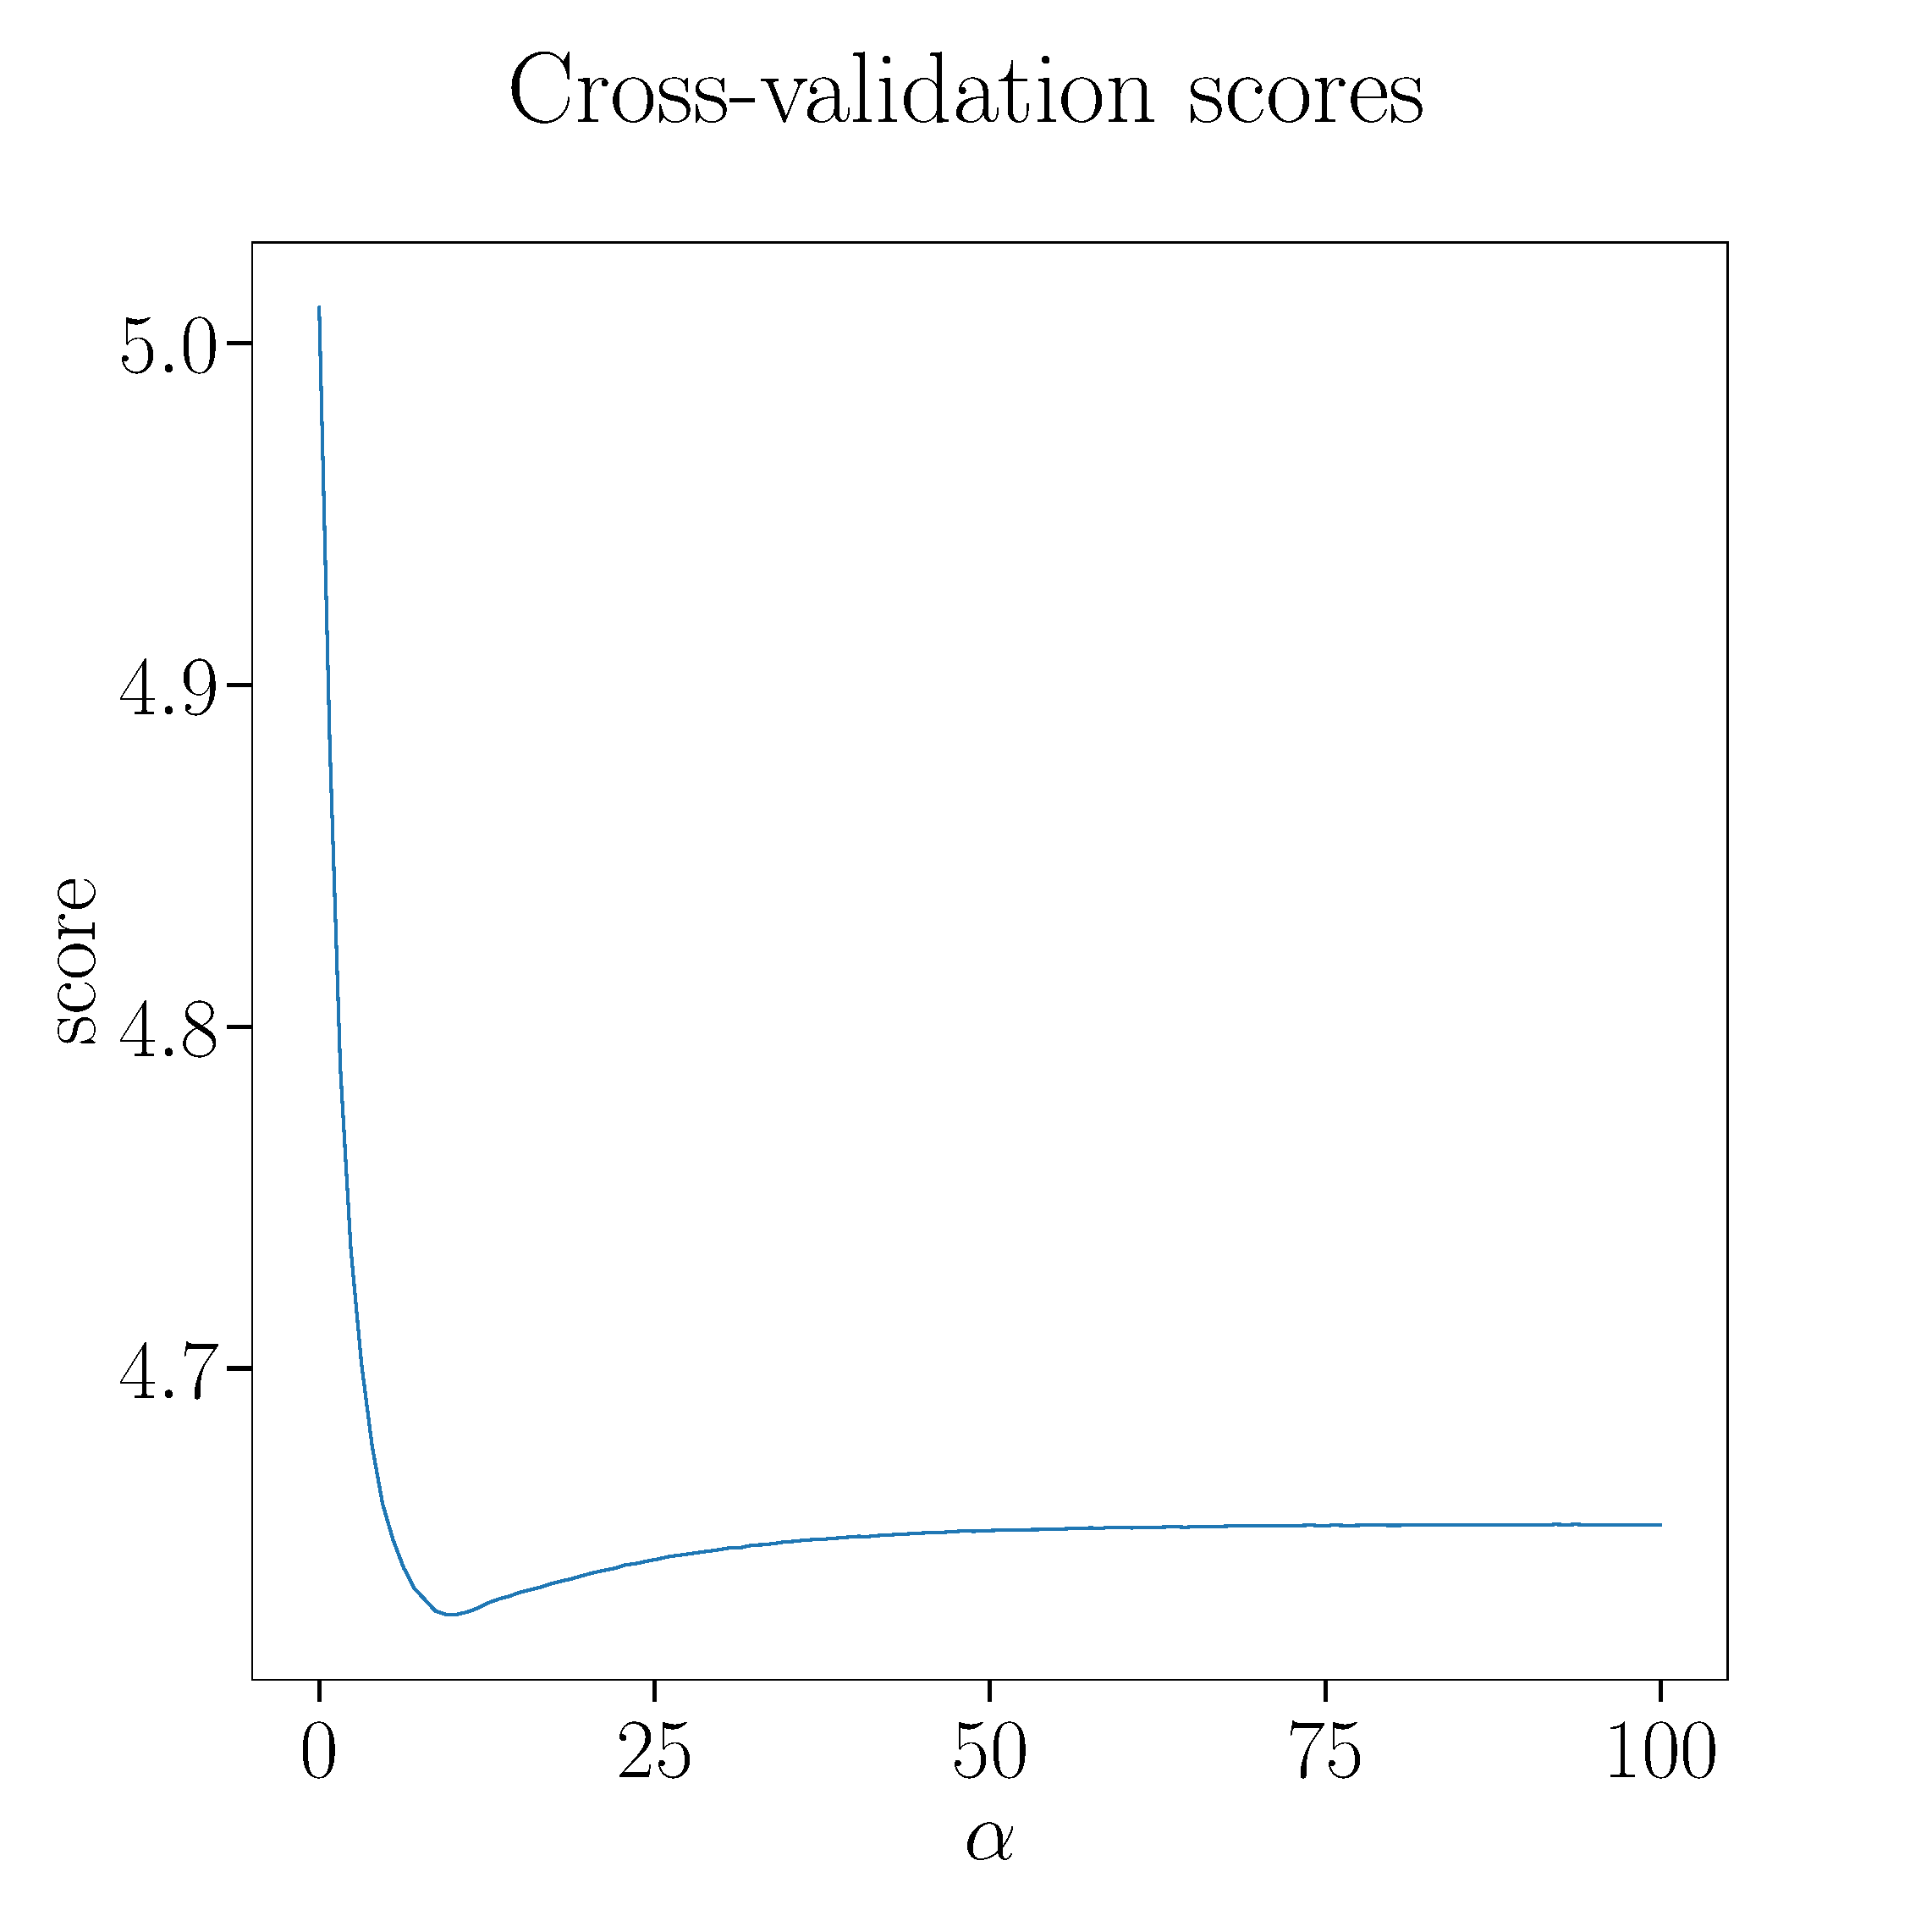
\includegraphics[width=.5\textwidth]{./figures_tex/cv_score}
		\end{center}
		\caption{Score function (\ref{ex2:score-function}) evaluated for a range of $\alpha$ values.}
		\label{ex2:score-graph}
	\end{figure}

	One can see that the minimum score is achieved at
	\begin{align}
		\hat{\alpha} = \underset{\alpha\in[0,100]}{\arg\min}f_\alpha\approx 10.
	\end{align}
	When evaluating the minimization problem (\ref{method:minimizationproblem}) with $\hat{\alpha}$ as hyperparameter for the regularizer and applying a cut-off of $10^{-10}$ to the yielded parameters, one obtains the simpler set of reactions $A\xrightarrow{\hat{k}_1}D$, $D\xrightarrow{\hat{k}_3} B$, and $A+B\xrightarrow{\hat{k}_4}C$ with rates as in Table \ref{tab:estimated-rates}.

	\begin{table}
		\centering
		\begin{tabular}{ccc}
			Reaction & original rate & estimated rate \\ \hline\noalign{\vskip .1cm}
			$A \to D$ & $k_1 = 2\cdot 10^{-2}$ & $\hat{k}_1 \approx 3.5\cdot 10^{-3}$\\
			$D \to A$ & $k_2 = 2\cdot 10^{-2}$ & $\hat{k}_2 = 0$ \\
			$D\to B$ & $k_3 = 1\cdot 10^{-2}$ & $\hat{k}_3\approx 9.1 \cdot 10^{-3}$ \\
			$A+B\to C$ & $k_4 = 1\cdot 10^{-4}$ & $\hat{k}_4\approx 8.7 \cdot 10^{-5}$ \\
			$C \to D+B$ & $k_5 = 1\cdot 10^{-4}$ & $\hat{k}_5 = 0$
		\end{tabular}
		\caption{Original and estimated reaction rates for the example in Section \ref{sec:ex2}.}
		\label{tab:estimated-rates}
	\end{table}

	One can see in Figure \ref{ex2:result} that with this simpler set of reactions the observed concentration curves can be explained as well. Further, it can be argued that the second reaction of the original model $D\xrightarrow{k_2}A$ is compensated by a smaller rate $\hat{k}_1 < k_1$ and that the fifth reaction of the generating model can be neglected altogether in the observed timescale as its rate is two orders of magnitude smaller than the other unimolecular reactions' rates.
	The parameters $k_3$ and $k_4$ are approximately recovered by $\hat{k}_3$ and $\hat{k}_4$, respectively.

	\begin{figure}
		\begin{center}
			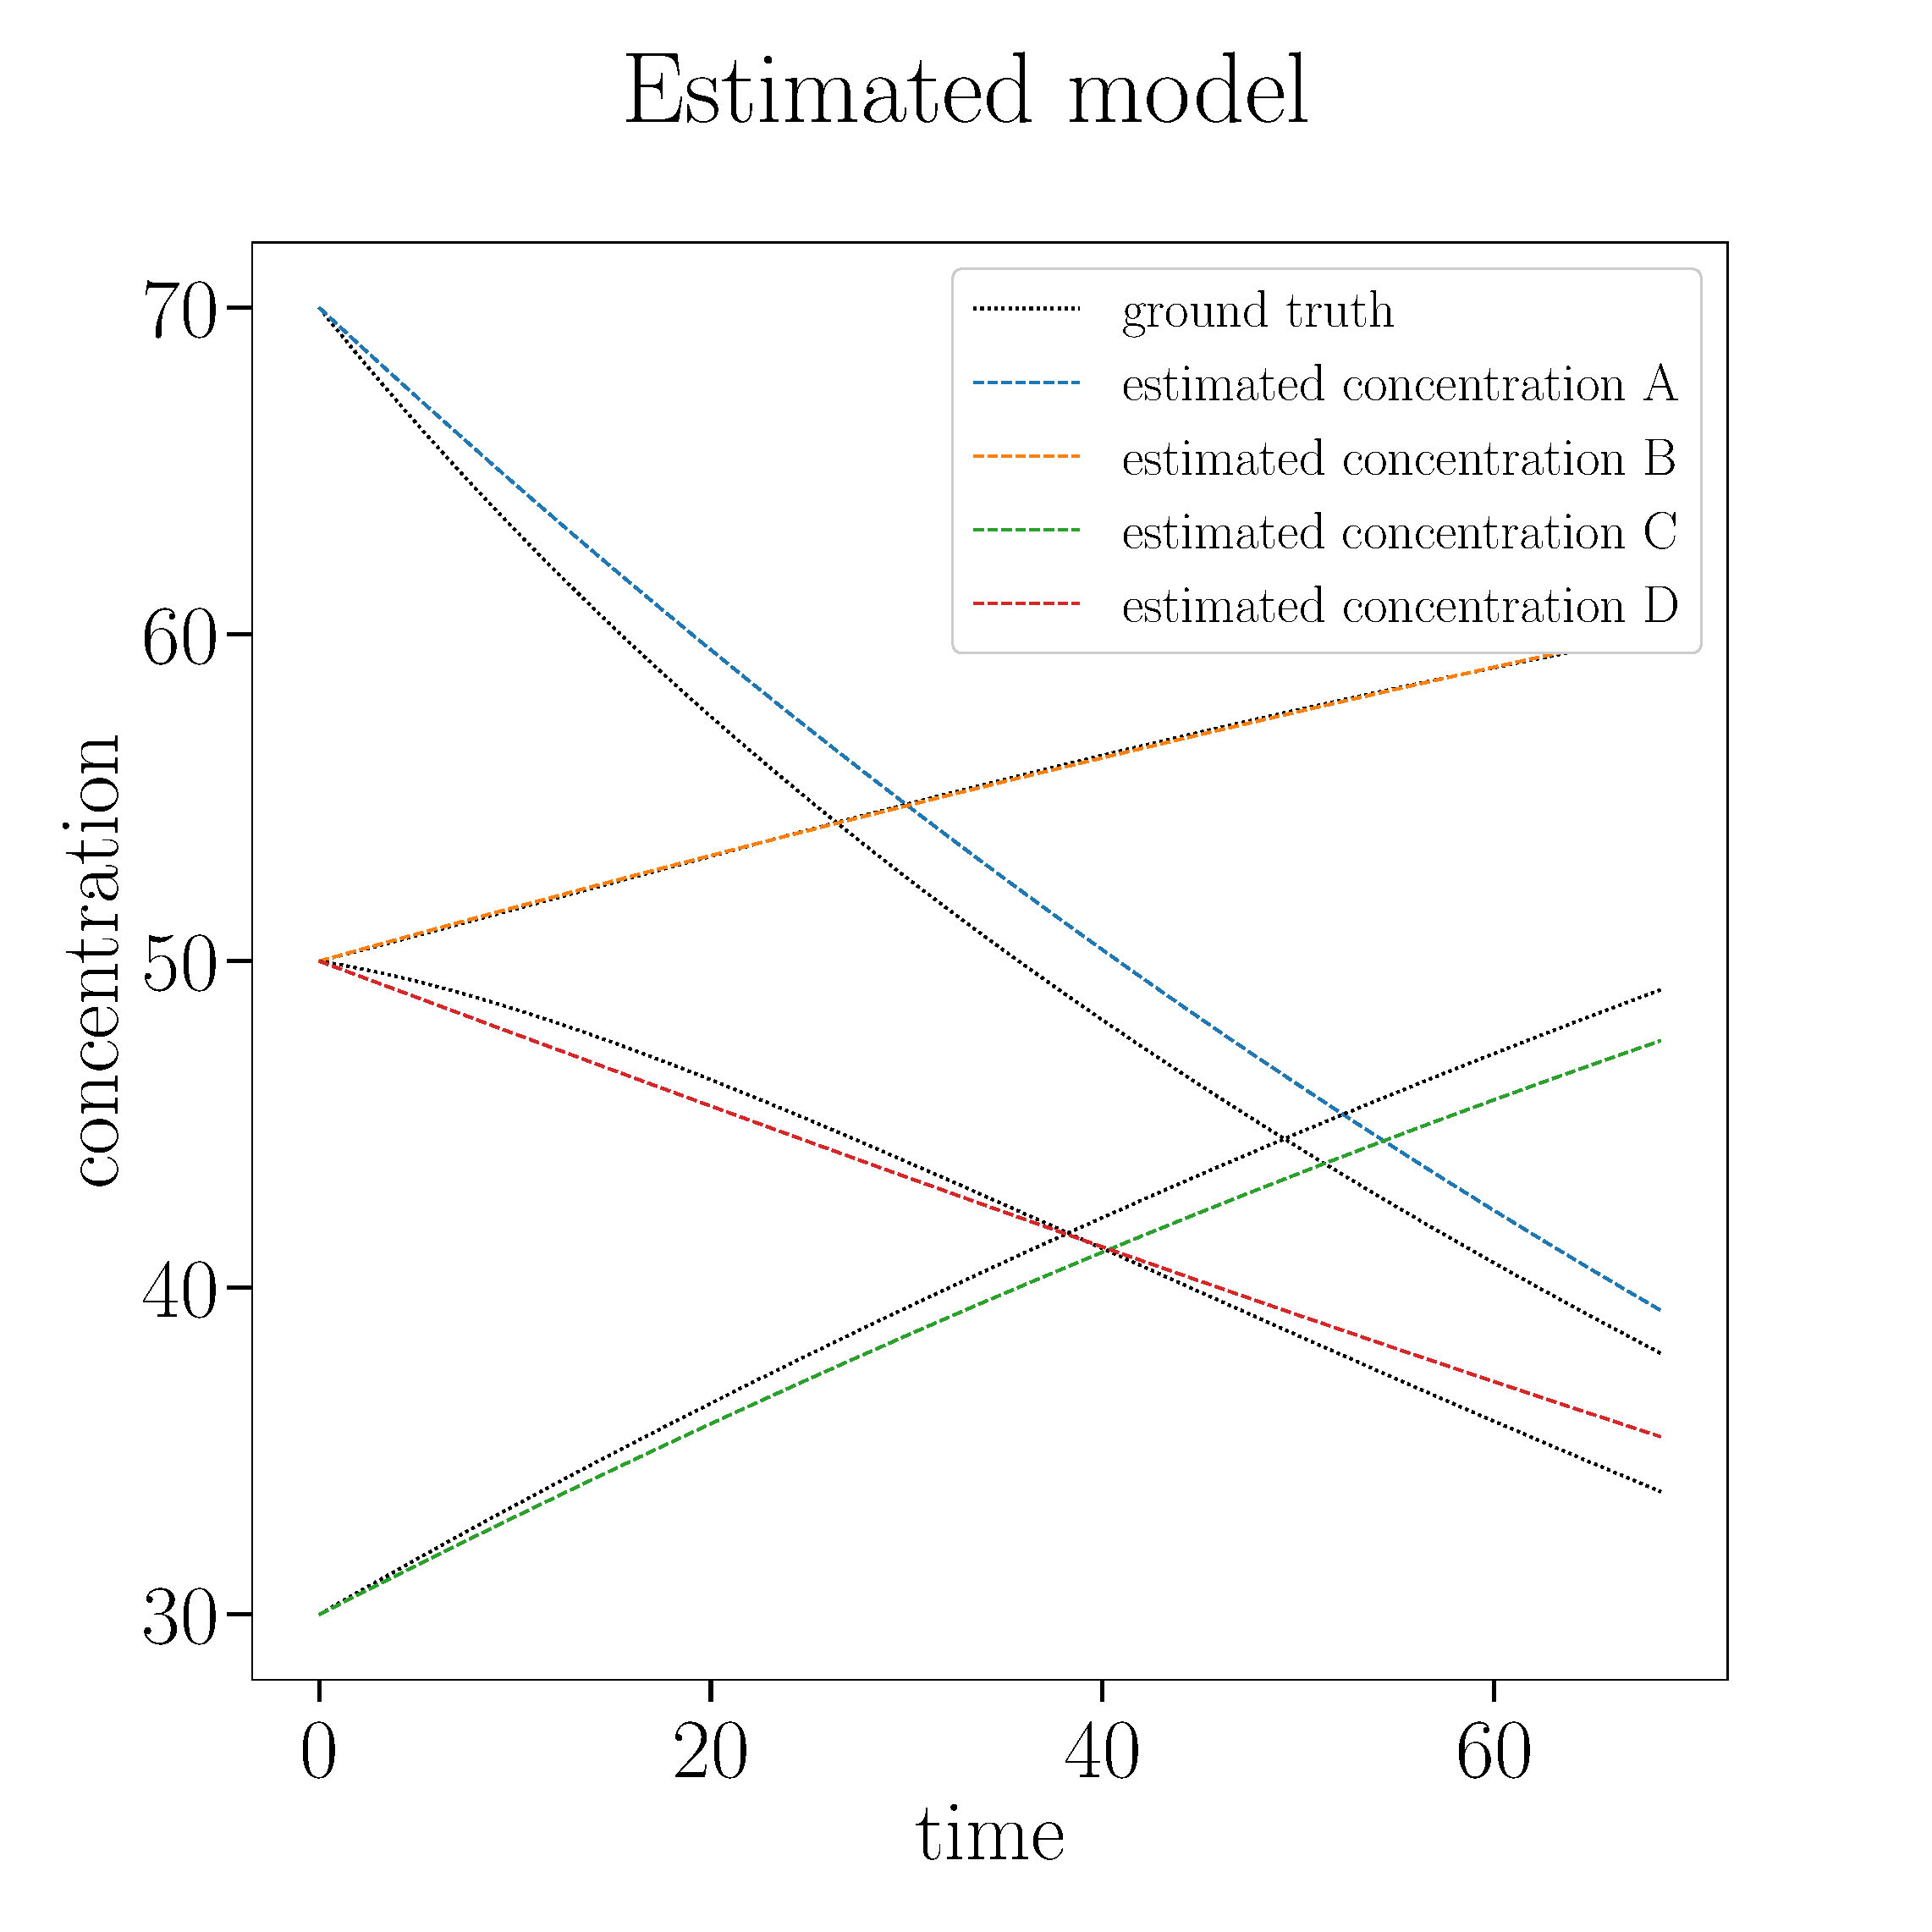
\includegraphics[width=.5\textwidth]{./figures_tex/cv_expected_estimated_concentrations}
		\end{center}
		\caption{Integrated law of mass action equations (\ref{method:the-system}) for the sparse estimated parameters and the corresponding Gillespie realization for the example in Section \ref{sec:ex2}.}
		\label{ex2:result}
	\end{figure}

	\section{Conclusion}
	In this work we have successfully applied and extended the SINDy method to not only parsimoniously detect potentially nonlinear terms in a dynamical system from noisy data, but also yield, in this case, a sparse set of rates with respect to generating reactions (\ref{method:the-reactions}).

	In two examples it was demonstrated that despite noisy data and unavailable derivative measurements, a parsimonious generating reaction network that is qualitatively able to explain the observed data can be estimated.
	In particular it was shown in the first example that if there is no ambiguity in the underlying model and ansatz reaction library, the actual rates can be recovered with decreasing time step, i.e., increasing resolution of the jump process.
	In the second example we could obtain an even simpler model than what was used to generate data by making use of sparse regression and cross-validation.

	\newpage
% 	\bibliographystyle{alpha}
	\bibliographystyle{abbrv}
	\bibliography{bibliography.bib}

\end{document}
